\section{Theory of HMMs}
\label{sec:theory}

\subsection{The 3 things you want from an HMM}
\label{sec:problems}

\begin{frame}
  
  The 3 fundamental problems \parencite{rabiner1989tutorial}
  \begin{itemize}
  	\item Particularization of temporal inference problems to the HMM case
  	\item The restricted structure of the HMM allows for elegant implementations of all the basic algorithms
  \end{itemize}
  \pause

  \begin{block}{Evaluation Problem}
    Given a model and a sequence of observations, how do we compute the probability that the \alert{observed 
    sequence} was produced by the model?
  \end{block}
  \pause
  \begin{block}{Best Explanation of Observations Problem}
    Given a model and a sequence of observations how do we choose a corresponding sequence of \alert{states} which 
    \emph{gives meaning} to the observations? How do we \emph{uncover} the hidden part of the model?
  \end{block}
  \pause
  \begin{block}{Model Estimation (Training) Problem}
    Given some observed sequences, how do we adjust the \alert{parameters} of an HMM model that best tries to explain 
    the observations? 
    
  \end{block}

\end{frame}


\subsection{Mathematical Foundations for HMMs}
\label{sec:math}


\begin{frame}
  \frametitle{An example problem: Emotional states}
  \begin{columns}[T]
    \column{0.58\textwidth}
    \only<1>{\framebox{
\includegraphics[width=\textwidth]{graphics/example/hmm-final-m.pdf}}}
    \only<2>{\framebox{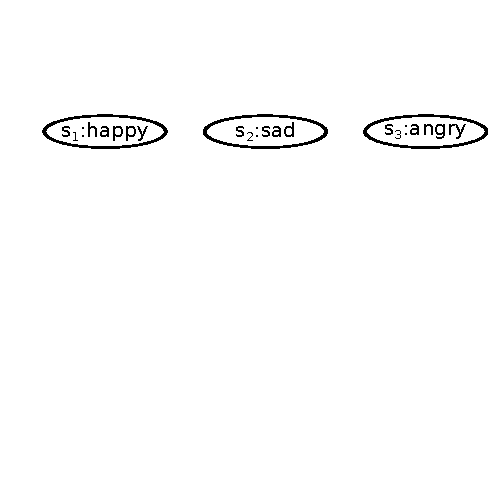
\includegraphics[width=\textwidth]{graphics/example/hmm-final-n.pdf}}}
    \only<3>{\framebox{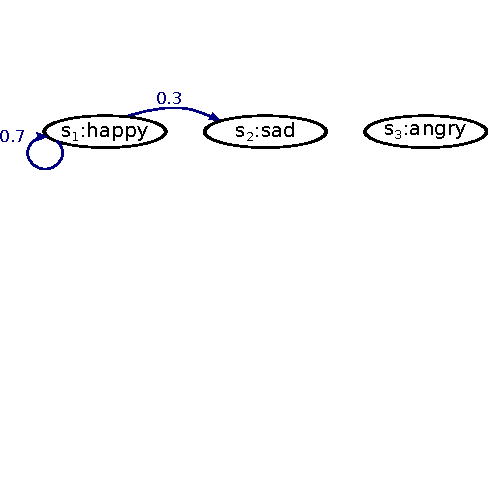
\includegraphics[width=\textwidth]{graphics/example/hmm-final-o.pdf}}}
    \only<4>{\framebox{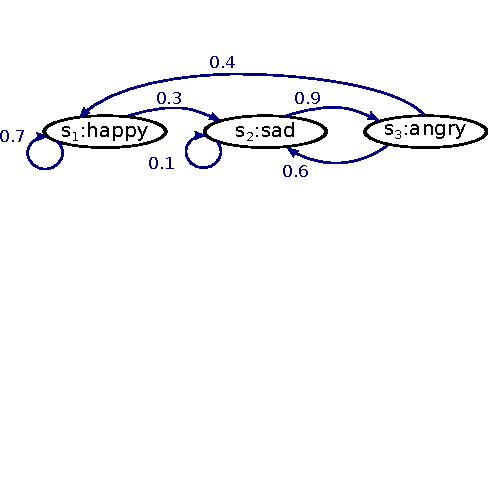
\includegraphics[width=\textwidth]{graphics/example/hmm-final-q.pdf}}}
    \only<5>{\framebox{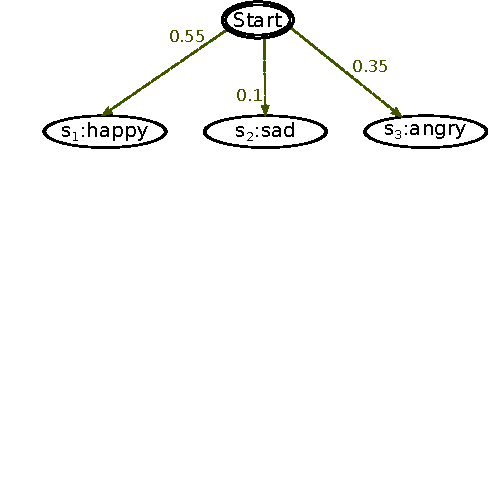
\includegraphics[width=\textwidth]{graphics/example/hmm-final-r.pdf}}}
    \only<6>{\framebox{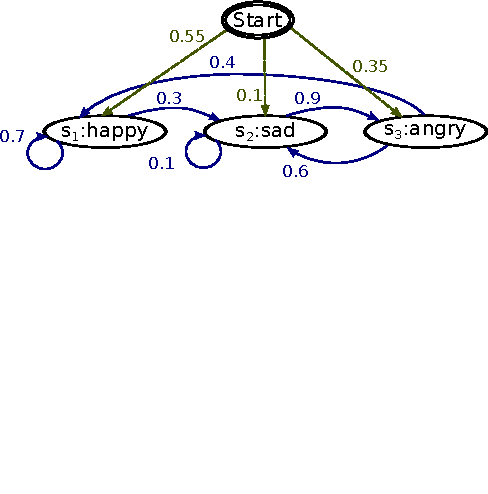
\includegraphics[width=\textwidth]{graphics/example/hmm-final-s.pdf}}}
    \only<7>{\framebox{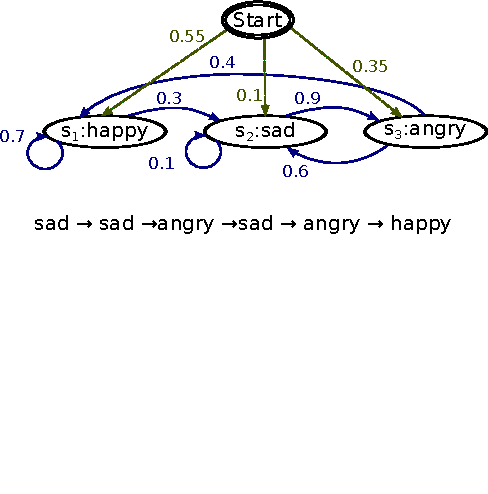
\includegraphics[width=\textwidth]{graphics/example/hmm-final-t.pdf}}}
    \only<8>{\framebox{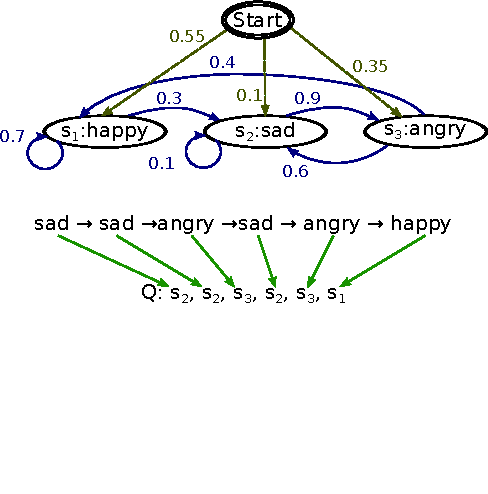
\includegraphics[width=\textwidth]{graphics/example/hmm-final-u.pdf}}}
    \only<9>{\framebox{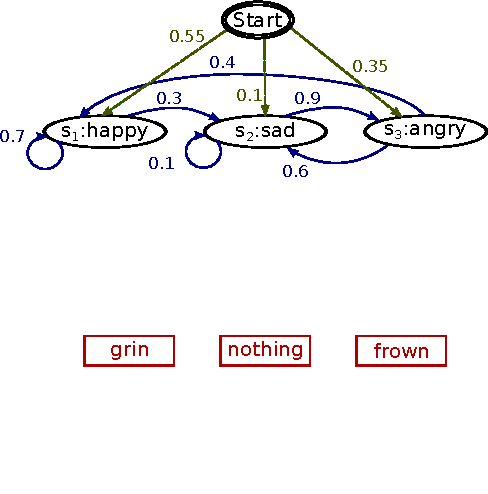
\includegraphics[width=\textwidth]{graphics/example/hmm-final-v.pdf}}}
    \only<10>{\framebox{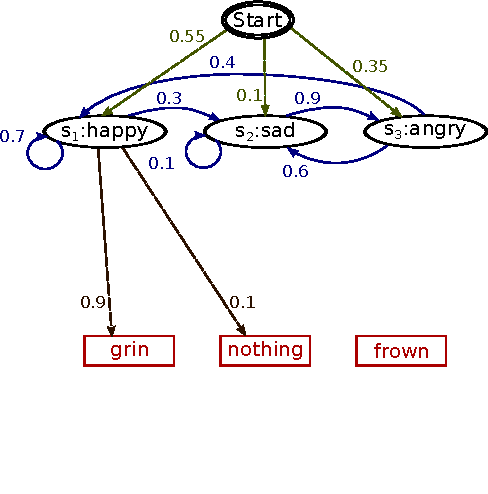
\includegraphics[width=\textwidth]{graphics/example/hmm-final-v2.pdf}}}
    \only<11-12>{\framebox{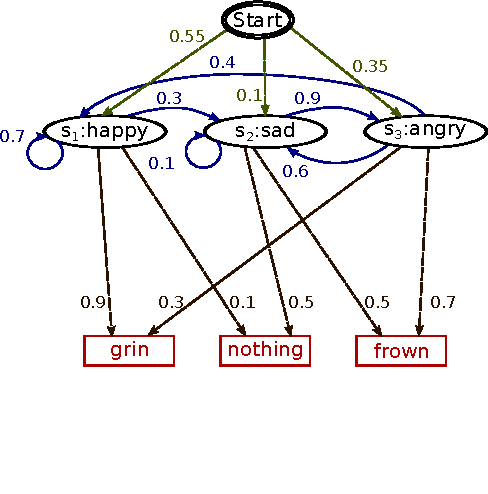
\includegraphics[width=\textwidth]{graphics/example/hmm-final-w.pdf}}}
    \only<13>{\framebox{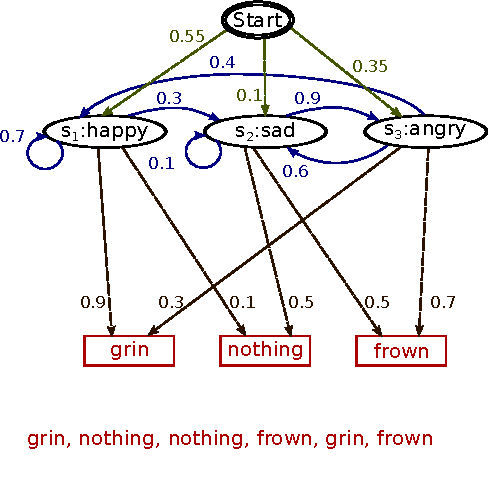
\includegraphics[width=\textwidth]{graphics/example/hmm-final-x.pdf}}}
    \only<14>{\framebox{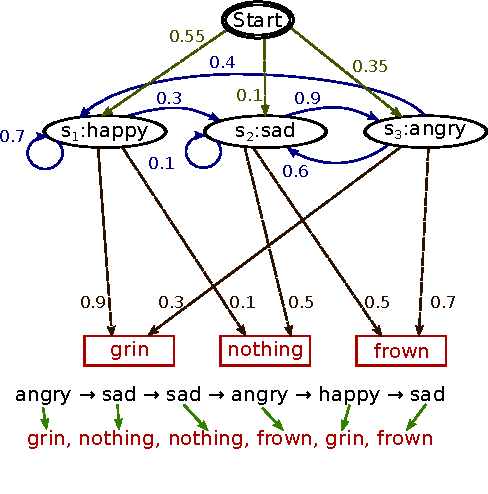
\includegraphics[width=\textwidth]{graphics/example/hmm-final-y.pdf}}}
    \only<15>{\framebox{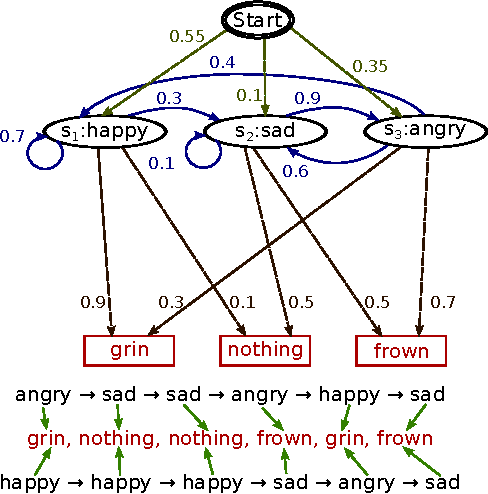
\includegraphics[width=\textwidth]{graphics/example/hmm-final-z.pdf}}}
    \only<16> {
      \begin{itemize}
      \item Example inspired from: \\\vspace*{1em}
        \fullcite{zubek2006introduction}
      \end{itemize}

    }
    

    \column{0.4\textwidth} \only<1>{ Let's consider a simple example:
      \\ \ a robot that tracks the emotional states of a player.  }
    \only<2>{ $\mathbf{N}$ - number of states \\ \vspace*{.5em}
      $\mathbf{N}=3$ \\ \vspace*{.5em} states:
      \begin{itemize}
      \item $s_1$: happy
      \item $s_2$: sad
      \item $s_3$: angry
      \end{itemize}

    }\only<3-4> { $\mathbf{A}$ - state transition probability
      distribution \\ \vspace*{.5em} \small{ $\mathbf{A} = \lbrace
        a_{i,j} \rbrace, \: 1 \le i, j \le N$ \\ \vspace*{.5em}
        $a_{i,j} = P(q_{t+1}=s_j \vert q_t = s_i)$
        \begin{itemize}
        \item $a_{\mathbf{1},1} = 0.7$
        \item $a_{\mathbf{1},2} = 0.3$
        \item $a_{\mathbf{1},3} = 0$
        \end{itemize}
        $\displaystyle\sum_{j=1}^{N}a_{i,j}=1, \quad 1 \le i \le N$ }
      \visible<4-> { $\mathbf{A} = \bordermatrix{~ & s_1 & s_2 & s_3
          \cr s_1 & 0.7 & 0.3 & 0 \cr s_2 & 0 & 0.9 & 0.1 \cr s_3 &
          0.4 & 0.6 & 0 \cr}$ }

    }
    
    \only<5>{ $\mathbf{\Pi}$ - initial state distribution \\
      \vspace*{0.5em} $\mathbf{\Pi} = \lbrace \pi_i \rbrace,\quad 1
      \le i \le N$ \\ \vspace*{0.5em} $\pi_i = P(q_1 = s_i)$ \\
      \vspace*{0.5em}
      
      $ \mathbf{\Pi} = \bordermatrix{ ~ & s_1 & s_2 & s_3 \cr ~ & 0.35
        & 0.1 & 0.55 \cr} $ }
    
    \only<6-8>{ $A = \bordermatrix{~ & s_1 & s_2 & s_3 \cr s_1 & 0.7 &
        0.3 & 0 \cr s_2 & 0 & 0.9 & 0.1 \cr s_3 & 0.4 & 0.6 & 0 \cr}$
      \\ \vspace*{0.25em} $\Pi = \bordermatrix{ ~ & s_1 & s_2 & s_3
        \cr ~ & 0.35 & 0.1 & 0.55 \cr}$ \\ \vspace*{0.25em}
      \visible<8> { $Q = [ q_1 q_2 \cdots q_T ]$ \small{
          \begin{equation*}
            \begin{split}
              P(Q & \vert A,\Pi)= \\ & = \pi_{q_1}a_{q_1,q_2}\cdots
              a_{q_{T-1},q_T}
            \end{split}
          \end{equation*}
          \begin{equation*}
            \begin{split}
              P(s_2,s_2,s_3,s_2,s_3,s_1\vert A,\Pi) = \\
              = \pi_2 \cdot a_{2,2} \cdot a_{2,3} \cdot a_{3,2} \cdot a_{2,3} \cdot a_{3,1} \\
              = \scriptstyle{0.1 \cdot 0.3 \cdot 0.1 \cdot 0.9 \cdot 0.6 \cdot 0.9 \cdot 0.4} \\
              = \scriptstyle{0.0005832}
            \end{split}
          \end{equation*}
        } }}

    \only<9>{ $\mathbf{M}$ - number of distinct observable values \\
      \vspace*{.5em} $\mathbf{M}=3$ \\ \vspace*{.5em} values:
      \begin{itemize}
      \item $v_1$: grin
      \item $v_2$: nothing
      \item $v_3$: frown
      \end{itemize}
    }

    \only<10-11> { $\mathbf{B}$ - observation values probability
      distribution \\ \vspace*{.5em} \small{ $\mathbf{B} = \lbrace
        b_{j,k} \rbrace \: \scriptstyle{1 \le j \le N, 1 \le k, \le
          M}$
        \begin{equation*}
          \begin{split}
            b_{j,k} & =b_{j}(v_k) \\
            & =P(o_t = v_k \vert q_t = s_j)
          \end{split}
        \end{equation*}
        \vspace*{-1.5em} \scriptsize{
          \begin{itemize}
          \item $b_{\mathbf{1},1} = b_{\mathbf{1}}(grin) = 0.9$
          \item $b_{\mathbf{1},2} = b_{\mathbf{1}}(nothing) = 0.1$
          \item $b_{\mathbf{1},3} = b_{\mathbf{1}}(frown) = 0$
          \end{itemize}}
        $\displaystyle\sum_{k=1}^{M}b_{j,k}=1, \quad 1 \le j \le N$\\
      }\visible<11> { $\mathbf{B} = \bordermatrix{ ~ & grin & notg &
          frown \cr s_1 & 0.9 & 0.1 & 0 \cr s_2 & 0 & 0.5 & 0.5 \cr
          s_3 & 0.3 & 0 & 0.7 \cr }$ } }
    
    \only<12>{ $\mathbf{\lambda}$ - parameters of the model \\
      \vspace*{.5em} $\lambda = (A, B, \Pi)$ \\ \vspace*{2em} $A$ -
      state transition probability distribution \\ \vspace*{.5em} $B$
      - observation values probability distribution \\ \vspace*{.5em}
      $\Pi$ - initial state distribution }
    
    \only<13-15>{ $\mathbf{O}$ - observation sequence \\ \vspace*{1em}
      $\mathbf{T}$ - length of observation sequence \\ \vspace*{1em}
      $O = [ o_1 o_2 \cdots o_T ]$ }

  \end{columns}
\end{frame}

\begin{frame}[T]
  \frametitle{Restating the three fundamental HMM Problems}
  
  \begin{block}{Evaluation Problem}
    Given a model \visible<2->{\alert{$\lambda=(A,B,\Pi)$}} and a
    sequence of observations \visible<3->{\alert{$O = [ o_1 o_2 \cdots
        o_T ]$}}, how do we compute the probability
    \visible<4->{\alert{$P(O \vert \lambda)$}} that the
    observed sequence was produced by the model? \\
  \end{block}
  \visible<5->{
  
    \begin{itemize}
    \item Enumerate every possible state sequence:

      \begin{equation}
        \begin{split}
          P(O \vert \lambda) = \displaystyle\sum_{\text{all}\;Q} P(O
          \vert Q, \lambda) \cdot P(Q \vert \lambda)
        \end{split}
        \label{eq1}
      \end{equation}
    \end{itemize}
    
  }
\end{frame}

\begin{frame}
  \frametitle{Restating the three fundamental HMM Problems}
  \begin{equation}
    \begin{split}
      P(O \vert \lambda) = \displaystyle\sum_{\text{all}\;Q} P(O \vert
      Q, \lambda) \cdot P(Q \vert \lambda)
    \end{split}
    \tag{\ref{eq1}}
  \end{equation}
  \pause \vspace*{.em}
  \begin{equation}
    P(O \vert Q, \lambda) = \displaystyle\prod_{t=1}^{T} P(o_t \vert
    q_t, \lambda)= \displaystyle\prod_{t=1}^{T} b_{q_t}(o_t) =
    b_{q_1}(o_1) \cdot \ldots \cdot b_{q_T}(o_T)
    \label{eq:pql}
  \end{equation}\pause
  \vspace*{.em}
  \begin{equation}
    P(Q | \lambda) = \pi_{q_1}\displaystyle\prod_{t=2}^{T}
    a_{q_{t-1},q_t} = \pi_{q_1} \cdot a_{q_1,q_2} \cdot a_{q_2,q_3} \cdot \ldots \cdot
    a_{q_{T-1},q_T}\label{eq:pql2}
  \end{equation}\pause
  \vspace*{.em}
  \begin{equation}
    \begin{split}
      P(O \vert \lambda) = \displaystyle\sum_{all\;Q} P(O, Q \vert
      \lambda) & = \displaystyle\sum_{all\;Q} P(O,\vert Q, \lambda)
      \cdot P(Q, \lambda) \\
      & = \displaystyle\sum_{\text{all}\;Q} \Big( \pi_{q_1} \cdot
      b_{q_1}(o_1) \cdot \displaystyle\prod_{t=2}^{T} b_{q_t}(o_t)
      a_{q_{t-1},q_t} \Big)
    \end{split}
    \tag{\ref{eq1}}
  \end{equation}
\end{frame}

\begin{frame}
  \frametitle{Restating the three fundamental HMM Problems}
  \begin{block}{Best Explanation of Observations Problem}
    Given a model \visible<2->{\alert{$\lambda=(A,B,\Pi)$}} and a
    sequence of observations \visible<3->{\alert{$O = [ o_1 o_2 \cdots
        o_T ]$}} how do we choose a corresponding sequence of
    \alert{states} \visible<4->{\alert{$Q = [ q_1 q_2 \cdots q_T ]$}}
    which \emph{gives meaning} to the observations?  How do we
    \emph{uncover} the hidden part of the model?
  \end{block}
  \visible<5->{
    \begin{itemize}
    \item There is no single answer.
    \item The sequence of individually most likely states:
      \begin{equation}
        \label{eq:inidi}
        Q_{\text{best}} = [\hat{q}_1\; \hat{q}_2\; \ldots \hat{q}_T], 
        \quad \hat{q}_t = \underset{s_i}{argmax}\; P(q_t = s_i \vert O, \lambda)
      \end{equation}
      
    \visible<6->{\item The best path
      \begin{equation}
        Q_{\text{best}} = \underset{Q}{\operatorname{argmax}}\;
        P(Q \vert O, \lambda)
        = \underset{Q}{\operatorname{argmax}}\; P(Q, O \vert \lambda)
        \label{eq:best-explanation}
      \end{equation}}
    \end{itemize}
  }
\end{frame}




\begin{frame}
  \frametitle{Restating the three fundamental HMM Problems}
  \begin{block}{Model Estimation (Training) Problem}
    Given some observed sequences \visible<2->{\alert{$\mathcal{O} =
        [O_1 O_2 \cdots O_L]$}}, how do we adjust the
    \alert{parameters} \visible<3->{\alert{$\lambda=(A,B,\Pi)$}} of an
    HMM model that best tries to explain the observations?
  \end{block}
  \visible<4->{
    \begin{itemize}
    \item The above question can be asked formally:
      \begin{equation}
        \lambda_{\text{best}} = \underset{\lambda}{\operatorname{argmax}}\;
        P(\mathcal{O} \vert \lambda)
        \label{eq:best-explanation}
      \end{equation}
    \end{itemize}
  }
\end{frame}



\subsection{Notation Conventions \& Framework Description}
\label{sec:octave}

\begin{frame}
  \frametitle{Notation Conventions}

  
\end{frame}


\begin{frame}
  \frametitle{Variables in Octave}

  
\end{frame}
